\documentclass{homework651}
% \usepackage{cmacros}
%% Feel free to add your own commonly used commands to this file.

\newcommand{\Reals}{\ensuremath{\mathbb R}}% Gives you a shortcut for writing the blackboard R for the real numbers - \RR
\newcommand{\Nats}{\ensuremath{\mathbb N}} % Gives you a shortcut for writing the blackboard N for the natural numbers - \NN
\newcommand{\Ints}{\ensuremath{\mathbb Z}} % Gives you a shortcut for writing the blackboard Z for the integer numbers - \ZZ
\newcommand{\Rats}{\ensuremath{\mathbb Q}} % Gives you a shortcut for writing the blackboard Q for the rational numbers - \QQ
\newcommand{\Cplx}{\ensuremath{\mathbb C}} % Gives you a shortcut for writing the blackboard C for the complex numbers - \CC

% Make better absolute value bars and the norm symbol
\newcommand{\abs}[1]{\left|#1\right|}
\newcommand{\norm}[1]{\left|\left|\,#1\,\right|\right|}

%% Now make some equivalents that some people may prefer.
\let\RR\Reals
\let\NN\Nats
\let\II\Ints
\let\CC\Cplx
\let\ZZ\Ints

%Add a shortcut for \rightarrow
\let\ra\rightarrow

%Add a \diam command for diameter
\newcommand{\diam}{\text{diam}}

\def\ra{\rightarrow}
\def\Reals{\mathbb{R}}
\def\SS{\mathbb{S}}
\usepackage{graphicx}
% \usepackage{wrapfig}
\usepackage[all,cmtip]{xy}
\geometry{top=1in, bottom=0.75in, left=1in, right=1in}


\doclabel{Math F651: Take Home Midterm}
\docauthor{Stefano Fochesatto}
\docdate{ March 10, 2023 }

\begin{document}


\begin{problems}
\problem A subset $A$ of a topological space $X$ is said to be nowhere dense if $\mathrm{Int}\; \overline{A} = \emptyset$.
\begin{subproblems}
\item Let $U$ be an open subset of a topological space. Prove that $\partial U$ is closed and nowhere dense.
\begin{proof} Suppose $U$ is an open subset of $X$. Clearly $\partial U$ is closed as its defined as an intersection of 
    closed sets, $\partial U = \overline{U} \cap \overline{U^c}$. Note that $\Int \overline{\partial U} = \Int \partial U$ since $\partial U$ is closed.
    Suppose for the sake of contradiction that $x \in U' \subseteq \partial U$ is open. Since $U$ is open and $\partial U \subseteq \overline{U^c} = U^c$ it follows that that $U \cap \partial U = \emptyset$. 
    By definition $x \not \in \overline{U}$ since $x \in U'$ such that $U'\cap U = \emptyset$ i.e $x$ is not a contact point of $U$, a contradiction.
\end{proof}
\item Let $V$ be a closed and nowhere dense set. Show that $V$ is the boundary of an open set.
\begin{proof}
    Suppose $V$ is closed an $\Int V = \emptyset$. Note that $V^c$ is an open set with the property that $\partial V^c = (\overline{V^c} \cap \overline{(V^c)^c}) = (\overline{V^c} \cap \overline{V})$. 
    Let $x \in V$ and note that since $\Int V = \emptyset$ it follows that $x$ is 
    a contact point to $V^c$. So $x \in \overline{V^c}$ and since $x \in \overline{V}$ we conclude that $x \in \partial V^c$.
    
    Let $x \in \partial V^c$. By definition $x \in \overline{(V^c)^c} = \overline{V} = V$. Thus $V = \partial V^c$.
\end{proof}
\end{subproblems}


\problem Let $f$ and $g$ be continuous maps from a topological space $X$ to a Hausdorff
space $Y$.  Suppose $f=g$ on a dense subset of $X$. Prove that $f=g$. 
\begin{proof} Let $f$ and $g$ be continuous maps from a topological space $X$ to a Hausdorff
    space $Y$.  Suppose $f=g$ on a dense subset $X' \subseteq X$. For the sake of contradiction suppose that for some $x \in X$ $f(x) \neq g(x)$. 
    Since $Y$ is Hausdorff, there exists open sets $f(x) \in U_f$ and $g(x) \in U_g$ such that $U_f \cap U_g = \emptyset$. Since $f$ and $g$ are continuous 
    we know that $f^{-1}(U_f)$ and $g^{-1}(U_g)$ are open in $X$. Note that $x \in f^{-1}(U_f) \cap g^{-1}(U_g) = U$, and since $X'$ is dense in $X$ there exists an $x' \in U$
    such that $f(x') = g(x')$. Note that $x' \in f^{-1}(U_f)$ and $x' \in g^{-1}(U_g)$ so it follows that $f(x') \in U_f$ and $g(x') \in U_g$. Therefore $f(x') \in U_f \cap U_g$ a contradiction. 
\end{proof}





\problem {\color{blue} Exercise 4.38} Let $X$ be a compact space, and suppose $\{F_n\}$
is a countable collection of nonempty closed subsets of $X$ what are nested, which means that $F_n \subseteq F_{n+1}$
for each $n$. Show that $\cap_nF_n$ is nonempty. 

\begin{proof}Let $X$ be a compact space, and suppose $\{F_n\}$
    is a countable collection of nonempty closed subsets of $X$ what are nested, which means that $F_n \subseteq F_{n+1}$
    for each $n$. For the sake of contradiction suppose $\cap_nF_n = \emptyset$ which is equivalent to showing $\cap_n(F_n)^c = X$. Note that the set $\{(F_n)^c\}$
    is an open cover of $X$ and therefore has a finite subcover $\mathcal{U} = \{F_\alpha\}_{\alpha \in A}$. Since $\mathcal{U}$ is finite there exists a largest element $F_k^c$, and by construction we know that
    \begin{equation*}
        F_k^c \supseteq F_{k - 1}^c \supseteq ... \supseteq F_{0}^c
    \end{equation*}  
    So it follows that, $F_k^c =  \cup_{\alpha \in A} F_\alpha^c = X$ and therefore $F_k = \emptyset$ a contradiction.
    (this is a proof by contrapositive in disguise.) 

\end{proof}








\problem Suppose $X$ and $Y$ are spaces and $Y$ is compact.
Show that the projection $\pi: X\times Y \to X$ is a closed map.
\begin{proof} Suppose $X$ and $Y$ are spaces and $Y$ is compact. Let $U$ be a closed set in $X \times Y$. Note that to show $\pi(U)$ is closed it is 
    sufficient to show that $\pi(U)^c$ is open. Note that $U^c \subseteq \pi^{-1}(\pi(U))^c = \pi^{-1}(\pi(U)^c)$. Let $x \in \pi(U)^c$, and note that $U^c$
    is an open set in $X \times Y$ containing $\{x\}\times Y$. By the tube lemma there exists an open $V$ in $X$ such that $V \times Y \subseteq U$, which implies 
    that since $\{x\} \times Y \subseteq V \times Y$ then $V \times Y \subseteq \pi^{-1}(\pi(U)^c)$ which implies that $x \in V \subseteq \pi(U)^c$. Therefore $\pi(U)^c$ is an open set and thus $\pi(U)$ is closed. 
\end{proof}





\problem Let $G$ be an algebraic group.  We say that $G$ is a {\bf topological group}
if in addition $G$ is a topological space
such that that the multiplication
map $m:G\times G\ra G$ and the inversion map $i:G\ra G$ defined by $m(g,h)=g\cdot h$ and $i(g)=g^{-1}$
are continuous.



\begin{subproblems}
\item
Suppose $G$ is an algebraic group and a $T_1$ topological space.  Show that $G$ is a 
topological group if and only if the map $f:G\times G\ra G$ defined by $f(g,h)=g h^{-1}$
is continuous.
\begin{proof} $(\Rightarrow)$ Let $G$ be an algebraic group and a topological space. Suppose $G$
    is a topological group. By definition $m:G\times G\ra G$ and the inversion map $i:G\ra G$ defined by $m(g,h)=g\cdot h$ and $i(g)=g^{-1}$
    are continuous. Note that the map $f:G\times G\ra G$ defined by $f(g,h)=g h^{-1}$, is equivalent to $f(g, h) = m(g, i(h))$ and since 
    the components of $m(g, i(g))$ are continuous so is $f$.\\



    $(\Leftarrow)$ Let $G$ be an algebraic group and a topological space. Suppose the map $f:G\times G\ra G$ defined by $f(g,h)=g h^{-1}$
    is continuous. Note that the inversion map $i:G\ra G$ defined $i(g)=g^{-1}$ is equivalent to $i(g) = f(f(g,g), g) = gg^{-1}g^{-1} = g^{-1}$.
    Since $i(g)$ is a composition of continuous functions, it is also continuous. Note that the multiplication
    map $m:G\times G\ra G$ defined by $m(g,h)=g\cdot h$ is simply $m(g, h) = f(g, i(h)) = gh^{-1}$. Since $h(g, h)$ is a composition of continuous functions, it is also continuous.
    Thus $G$ is a topological group. 
\end{proof}




\item Let $G$ be a topological group and let $H$ be a subgroup.  Show that $\overline H$ is
a subgroup.  Hint: that map $f$ from the previous part is continuous. 
% 😉
\begin{proof} Suppose $G$ is a topological group and let $H$ be a subgroup. 
    Let $a, b\in \overline{H}$. Note that since $H$ is a subgroup of $G$, $f(H \times H) \subseteq H$ and since $H \subseteq \overline{H}$ it follows that 
    $H \times H \subseteq f^{-1}(\overline{H})$. Since $\overline{H}$ is closed and $f$ is a continuous function, $f^{-1}(\overline{H})$ is closed. Therefore 
    it follows that $\overline{H \times H} \subseteq f^{-1}(\overline{H})$. Note that $\overline{H} \times \overline{H} \subseteq \overline{H \times H}$ since 
    for all $x = (x_1, x_2) \in \overline{H} \times \overline{H}$, we know that $x$ is a contact point of $H \times H$ because $x_1$ and $x_2$ are contact points of $H$. Hence $f(\overline{H} \times \overline{H}) = f\overline{H}$ and therefore $\overline{H}$ is a subgroup. 

\end{proof}
\end{subproblems}



\problem Let $\{x_n\}_n$ be a sequence in an arbitrary
product $\prod X_\alpha$. Show that $x_n\to x$ if 
and only if $\pi_\alpha(x_n)\to \pi_\alpha(x)$ for every $\alpha$.
Then show that this result is false if we assume
instead that $\prod X_\alpha$ is given the box topology.
\begin{proof} $(\Rightarrow)$ Let $\{x_n\}_n$ be a sequence in an arbitrary product $\prod_{\alpha \in A} X_\alpha$. Suppose that $x_n \to x$, and note that by definition
    we know that for all $U \in \mathcal{V}(x)$ there exists some $N$, such that for all $n \geq N$, $\{x_n\}_{n \geq N} \in U$. 
    Consider the sequence $\pi_\alpha(x_n)$ for some factor $\alpha$. Let $U' \in \mathcal{V}(\pi_\alpha(x))$, and note that $\pi^{-1}_\alpha(U')$ is an open set in $\prod_{\alpha \in A} X_\alpha$ under the product topology, so there exists some $N$ such that for all $n \geq N$, $\{x_n\}_{n \geq N} \in \pi^{-1}_\alpha(U')$ so therefore $\pi_{\alpha}(\{x_n\}_{n \geq N}) = \{\pi_{\alpha}(x_n)\}_{n \geq N} \subseteq U'$.
\end{proof}

\begin{proof}$(\Leftarrow)$ Let $\{x_n\}_n$ be a sequence in an arbitrary product $\prod_{\alpha \in A} X_\alpha$. Suppose $\pi_\alpha(x_n)\to \pi_\alpha(x)$ for every $\alpha$.
    Suppose $U \in \mathcal{V}(x)$ and since $\prod_{\alpha \in A} X_\alpha$ has the product topology we know that there exists a basic open set $U'$, with $x \in U'\subseteq U$
    of the form $U' = \cap_{j \in J} \pi_j^{-1}(U_j)$ for some finite $J \subseteq A$ with $U_j$ an open set in $X_j$.
    Note that for each $U_j$ there exists an $N_j$ such that for all $n \geq N_j$, $\{\pi_j(x_n)\}_{n \geq N_j} \subseteq U_j$. Since $J$ is finite, 
    there exists a maximal $N_j$, $N$ where for all $j \in J$, $\{\pi_j(x_n)\}_{n \geq N} \subseteq U_j$. Therefore it follows that $\{x_n\}_{n \geq N}  \subseteq  \{\pi_j^{-1}( \pi_j(x_n) )\}_{n \geq N} \subseteq \pi_j^{-1}(U_j)$, for all $j \in J$ hence $\{x_n\}_{n \geq N} \subseteq U' \subseteq U$. 
\end{proof}

Clearly the $(\Leftarrow)$ direction does not hold if $\prod_{\alpha \in A} X_\alpha$ is endowed with the box topology. Let $U \in \mathcal{V}(x)$ be the basic open set of $U = \cap_{j \in J} \pi_j^{-1}(U_j)$ for some infinite $J \subseteq A$. There would then exists no maximal $N$ in the set of all $N_j$.




\problem Show that the following topological spaces are not manifolds:
\begin{enumerate}
    \item[(a)] The union of the x-axis and the y-axis in $\RR^2$.
    \begin{proof} Let $S$ be the union of the x-axis and the y-axis in $\RR^2$. Consider the point $(0, 0) \in S$ and note that for every $U' \in \mathcal{V}((0,0))$ there exists an $r > 0$ such that $U \subseteq U'$ where $U = B_r((0, 0)) \cap S$ is open via the subspace topology.
        Suppose to the contrary that there exists a homeomorphism $f: U \to \RR^n$ for all $n \geq 2$. Let $U^* = U \setminus \{(0, 0)\}$
        and note that $f|_{U^*}: U^* \to \RR^n \setminus\{f((0, 0))\}$ is a homeomorphism. Note that $U^*$ is disconnected since $\{(x, y) \in \RR^2 : y > x\}\cap S$ and $\{(x, y) \in \RR^2 : y < x\}\cap S$ are open in $S$ and partition $U^*$. Clearly for all $n \geq 2$, $\RR^n \setminus\{f((0, 0))\}$ is connected, thus a contradiction. Therefore for all $n \geq 2$, $U \not\sim \RR^n$ and thus $U' \not\sim \RR^n$ so $S$ is not locally Euclidean dimension $n$.


    We will conclude by showing that $U' \not\sim \RR$, and therefore $S$ is not locally Euclidean of dimension 1. Suppose there exist
    a homeomorphism $f: U \to \RR$. Again it follows that $f|_{U^*}: U^* \to \RR^n \setminus\{f((0, 0))\}$ is a homeomorphism. Clearly 
    $U^*$ has 4 components, namely $(\RR^- \times \{0\} \cap U^*)$, $(\RR^+ \times \{0\} \cap U^*)$, $(\{0\}\times \RR^+ \cap U^*)$, and $(\{0\} \times \RR^- \cap U^*)$ whose images in $\RR \setminus \{f((0, 0))\}$ must be disjoint. Note that $f$ is a closed and open map and there are only 2 disjoint closed and open sets in $\RR \setminus \{f((0, 0))\}$, namely $(-\infty, f((0,0)))$ and $(f((0, 0)), \infty)$. Therefore $f$ is a homeomorphism which maps a pair of disjoint sets to the same set, a contradiction. Thus $U \not\sim \RR$ and therefore $U' \not\sim\RR$. 
    \end{proof}
    \item[(b)] The conical surface $C \subseteq \RR^3$ defined by 
    \begin{equation*}
        C = \{(x, y, z): z^2 = x^2 + y^2\}
    \end{equation*} 
    \begin{proof} Suppose for the sake of contradiction that $C$ is an $n$-manifold. Consider the point $p^* = (0, 0, 0)$ and note that for every every $U' \in \mathcal{V}(p)$ there exists an $r > 0$ such that $U \subseteq U'$ where $U = B_r(p^*) \cap C$ is open via the subspace topology. 
    Let $U^* = U \setminus \{p^*\}$. Since $C$ is a $n$-manifold there exists a homeomorphism $f:U \to \RR^n$, and therefore $f|_{U^*}: U^* \to \RR^n \setminus \{f(p^*)\}$ is also a homeomorphism. Note that $U^*$ is disconnected since $\{(x, y, z) \in \RR^3: z > 0\} \cap U^*$ and $\{(x, y, z) \in \RR^3: z < 0\} \cap U^*$ partition $U^*$ and are open via the subspace topology. Therefore it follows that $\RR^n \setminus \{f(p^*)\}$ is also disconnected, thus it must have been the case that $n = 1$ with $U \sim \RR$. So $C$ is a 1-manifold. 
    
    Now consider the set $C^+ = C \setminus \{(x, y, z) \in C: z > 0\}$. We will proceed by showing that the map $\pi:C^+ \to \RR^2 \setminus \{(0 ,0)\}$ defined by $\pi((x, y, z)) = (x, y)$ is homeomorphism. 
    First suppose $\pi((x, y, z)) = \pi((x_1, y_1, z_1))$ and by $\pi$ we know that $x = x_1$ and $y = y_1$, and since our domain is $C^+$
    $z = \sqrt{x^2 + y^2} = \sqrt{x_1^2 + y_1^2} = z_1$, so $f$ is injective. Let $(x, y) \in  \RR^2 \setminus \{(0 ,0)\}$ and note that by definition of $C^+$ we know that $(x, y , \sqrt{x^2 + y^2}) \in C^+$ and by $\pi$ we get $\pi((x, y , \sqrt{x^2 + y^2})) = (x, y)$. So $f$ 
    is a surjection. Note that the component maps of $\pi$ are simply the identity so they are continuous and thus $\pi$ is continuous. 
    Define $\pi:\RR^2 \setminus \{(0 ,0)\} \to C^+$ by $\pi^{-1}((x, y)) = (x, y,\sqrt{x^2 + y^2})$. Again this map has two component maps which 
    are the identity, and another defined by $\pi_z^{-1}(x, y) = \sqrt{x^2 + y^2}$ which is also continuous. 

    So $\pi:C^+ \to \RR^2 \setminus \{(0 ,0)\}$ is a homeomorphism, and since $\RR^2 \setminus \{(0 ,0)\}$ is a $2$-manifold, so is $C^+$. Finally we have that there exists a neighborhood $U_2$ of $p \in C^+$ which is homeomorphic to $\RR^2$ and since $p \in C$, and $C$ is a $1$-manifold there exists another neighborhood of $p$, $U_1$ homeomorphic to $\RR$. So 
    $U_2 \cap U_1$ is homeomorphic to both $\RR^2$ and $\RR$. 
    \end{proof}
\end{enumerate}

\problem Let $M = \SS^1 \times \RR$, and let $A = \SS^1 \times \{0\}$. Show that the space $M/A$ obtained by collapsing $A$
to a point is homeomorphic to the space $C$ of the previous problem, and thus is Hausdorff and second countable but not locally Euclidean.  
\begin{proof} Let $M = \SS^1 \times \RR$, and let $A = \SS^1 \times \{0\}$. Let $q: M \to M/A$ be the natural projection sending $M$ to it's equivalence class. To show that $M/A$ is homeomorphic to $C$ we will proceed by first exhibiting a function $f: M \to C$ which is continuous and constant on the fibers of $q$. Consider $f$ defined by $f(((x, y), z)) = (xz, yz, z)$. Clearly the components of this function are continuous from $\RR^3$ and hence continuous from the restriction $M$. Since it's component maps are continuous, $f$ is a continuous function. Suppose $q(x) = q(x')$ for $x \neq x'$, and note that this is only the case when $x, x' \in A$ and are therefore of the form $x = ((x, y), 0)$ and $x' = ((x', y'), 0)$ so clearly $f(x) = f(x')$. Thus $f$ descends to the quotient as continuous function $\hat{f}:  M/A \to C$ where $f(x) = \hat{f}(q(x))$.


    Now let $g: C \to M\setminus \{S^1\} \cup \{(1, 1, 0)\}$ be defined by
    \begin{equation*}
        g((x, y, z)) = \begin{cases}
            \left(\left(\frac{x}{\sqrt{x^2 + y^2}}, \frac{y}{\sqrt{x^2 + y^2}}\right), z\right) & (x, y, z) \in C^*\\
            ((1, 1), 0) & (x, y, z) \in S^1
        \end{cases}
    \end{equation*} 
    Note that as a map from $C^* \to M\setminus \{S^1\}$, $g$ has continuous component maps since $C^*$ excludes $(0, 0, 0)$ and thus $g$ is continuous restricted onto $C^*$. Note that any open set $U \in  M\setminus \{S^1\} \cup \{(1, 1, 0)\}$ has a pre-image, $g^{-1}(U) = U^* \cup \{(0,0,0)\}$ where $U^*$ is open in $C^*$ and therefore $g^{-1}(U)$ is open in $C$. Thus $g$ is continuous and there exists a continuous map $\hat{g}: C \to M/A$ defined by $\hat{g}(x) = q(g(x))$.

    Finally we must show that $\hat{f}$ and $\hat{g}$ are inverses, note that exhibiting an inverse
    is sufficient to show a bijection between $M/A \to C$. Note that $\hat{g}(\hat{f}(q(x))) = q(g(\hat{f}(x))) = q(g(f(x))) = q(x)$. 
\end{proof}


\begin{lemma}{1} Let $X$ be a topological space with $a, b, c \in X$. If there exists a path in $X$ from $a$ to $c$ and from $b$ to $c$, then there exists a path from $a$ to $b$. 
    \begin{proof} Suppose there exists a path in $X$ from $a$ to $c$ and from $b$ to $c$, so there are continuous function $f_a:I \to X$ and $f_b:I \to X$ with $f_a(0) = a$, $f_a(1) = c$, $f_b(0) = b$, and $f_b(1) = c$. Note that $[0, 1/2]$ and $[1/2, 1]$ are homeomorphic to $I$ by $g_a$ and $g_b$ respectively where $g_a(x) = 2x$ and $g_b(x) = -2(x - 1)$. Note that $[0, 1/2]$ and $[1/2, 1]$ form a finite closed cover of $I$ and since $f_a(g_a(1/2)) = f_a(1) = c = f_b(1) = f_b(g_b(1/2))$ by the glueing lemma there exists a continuous map $f:I \to X$ whose restrictions on $[0, 1/2]$ and $[1/2, 1]$
    is equal to $f_a(g_a(x))$ and $f_b(g_b(x))$. Note that $f$ is a path from $a$ to $b$ in $X$. 
    \end{proof}
\end{lemma}

\problem Let $X$ be a topological space, and let $CX$ be the cone on $X$. 
\begin{enumerate}
    \item{(a)} Show that $CX$ is path-connected
    \begin{proof} Recall that $CX$ is defined as the quotient space $(X \times [0, 1])/(X \times \{0\})$ and let $q: X \to CX$ be the natural projection of $X$ onto its equivalence classes. Note that to show that $CX$ is path-connected, by Lemma 1 it is sufficient to show that there exists a path from an $x \in X$ to some fixed $x \in X$. Let $c \in CX$ be the point whose identified by $c = q(X \times \{0\})$. Let $x \in CX$, and note that since $q$ is a surjection there exists some $(x', i) \in X \times [0, 1]$ with the property that $q((x', i)) = x$. we will proceed by exhibiting a continuous function $f: I \to X \times [0, 1]$ with the property that $f(0) = (x', i)$ and $f(1) = (x', 0)$, whose composition with $q$ will define the path from $x$ to $c$ in $CX$. Let $f(z) = (x',(1 - z)i)$ and note that $f$ is continuous since it's component maps are also continuous. Finally since $q$ is continuous we know that $q\circ f: I \to CX$ is continuous with the property that $q(f(1)) = q((x', 0)) = c$ and $q(f(0)) = q((x', i)) = x$. 
    \end{proof}



    \begin{lemma}{2} The product of locally (path-)connected spaces is locally (path-)connected. 
        Suppose $X$ and $Y$ are locally (path-)connected. Let $p \in X \times Y$ and consider $U \in \mathcal{V}(p)$. Note that by the product topology we know $U = \pi_x^{-1}(U_x) \cap \pi_y^{-1}(U_y)$ where $U_x$ and $U_y$ are open sets in $X$ and $Y$ respectively. Since $U_x$ and $U_y$ belong to locally (path-)connected spaces there exists (path-)connected sets $U'_x \subseteq U_x$ and $U'_y \subseteq U_y$ such that $\pi_x^{-1}(p) \in U'_x$ and $\pi_y^{-1}(p) \in U'_y$. Clearly $U' = U'_x \times U'_y$
        is (path-)connected, since it's a product of (path-)connected sets and also by construction has the property that $p \in U' \subseteq U$. Hence $X \times Y$ is locally (path-)connected. 
    \end{lemma}

    \item{(b)} Show that $CX$ is locally connected if and only if $X$ is, and locally path connected if and only if $X$ is. 

    \begin{proof}$(\rightarrow)$ Suppose $CX$ is locally (path-)connected. To show that $X$ is locally (path-)connected we will show that for any $p \in X$, $U \in \mathcal{V}(p)$ there exists an open (path-)connected subset $U'$ such that $p \in U' \subseteq U$. Let $p \in X$ and $U \in \mathcal{V}(p)$. Note that by the product topology, $U \times [0, 1]$ is open in $X \times [0, 1]$, and since $q$ is a quotient map it also must follow that $q(U \times [0, 1])$ is open in $CX$. Note that since $CX$ is locally (path-)connected there exists a (path-)connected set $CU' \subseteq q(U \times [0, 1])$ whose pre-image $q^{-1}(CU')$ is open in $X \times [0, 1]$ since $q$ is a quotient map and contains $p \times [0, 1]$. Let $U' = \pi_(q^{-1}(CU'))$ and note that by construction $p \in U' \subseteq U$. Thus $X$ is locally (path-)connected. 
        
    \end{proof}
    \begin{proof}$(\leftarrow)$ Suppose $X$ is locally path connected. By Lemma 2 we know that since $X$ is locally (path-)connected, $X \times (0, 1]$ is also locally (path-)connected. Since $q: X \times [0, 1] \to CX$ is a continuous map, it follows that the image $q(X \times (0, 1])$ is locally (path-)connected in $CX$. Let $v = q(X \times \{0\})$, what remains to be shown is that for any $U \in \mathcal{V}(v)$ there exists a (path-)connected subset $U'$ such that $v \in U' \subseteq U$. By the part (a) if this problem we know that $CX$ is path connected, so there must exists such a $U'$. Therefore $CX$ is locally (path-)connected.
    \end{proof}


\end{enumerate}

\problem Let $X$ be a topological space.  The {\bf suspension} of $X$, denoted by
$\Sigma X$, is the quotient of $X\times [-1,1]$ where all points of the form $(x,1)$
are identified, and all points of the form $(x,-1)$ are identified.  
Determine, with proof, a familiar space that is homeomorphic to $\Sigma S^n$.
\begin{proof}Consider $\Sigma S^n$, and note that by definition $\Sigma S^n$ is the quotient of $S^n\times [-1,1]$ where all points of the form $(x,1)$ are identified, and all points of the form $(x,-1)$ are identified. Let $q:S^n\times [-1,1] \to \Sigma S^n$ be the natural projection of $X\times [-1,1]$ onto its equivalence classes. Note that $S^n$ is compact, one can see that quickly by noting $S^n$ is closed and bounded and applying Heine-Borel. By Tychonoff's Theorem the product $S^n\times [-1,1]$ is compact. Now note that $S^{n+1}$ is a Hausdorff space, since for any $a, b\in S^{n+1}$ we can find a disjoint $a \in U_a$ and $b \in U_b$ in $\RR^{n+2}$ and by the subspace topology on $S^{n+1}$, $U_a\cap S^{n+1}$ and $U_b\cap S^{n+1}$ are open and disjoint. We will conclude by exhibiting a map surjective continuous map $f:S^n\times [-1,1] \to S^{n+1}$ which is closed via the closed map lemma and therefore a quotient map, showing that it makes the same identifications as $q$ and therefore by the uniqueness of quotient spaces $\Sigma S^n \sim S^{n+1}$.
    Let $f:S^n\times [-1,1] \to S^{n+1}$ be defined by $f((x, t)) = (\sqrt{1 - t^2}x, t)$. The component maps for $f$ are continuous from $\RR^{n+2}$ since the first is a nonzero scaling of a vector, and the second is a projection. Therefore $f$ is continuous on its domain and its image is $S^{n+1}$ since all for $(x, t) \in S^n\times [-1,1]$ we get $f((x, t)) = (\sqrt{1 - t^2}x, t)$ with,
    \begin{align*}
    |f((x, t))| &= |(\sqrt{1 - t^2}x, t)| = \left(\left(\sum_{i = 1}^{n+1} (\sqrt{1 - t^2}x_i)^2\right)  + t^2\right)^{1/2}\\ 
    &=  \left(\left(\sum_{i = 1}^{n+1} (1 - t^2)x_i^2\right)  + t^2\right)^{1/2}\\   
    &= \left((1 - t^2)\left(\sum_{i = 1}^{n+1}x_i^2\right)  + t^2\right)^{1/2}\\  
    &= \left(1 - t^2 + t^2\right)^{1/2} = 1.
    \end{align*}
    Let $(x_1, \dots, x_{n+2}) \in S^{n+1}$. Note that $f\left(\frac{1}{\sqrt{1 - x_{n+2}^2}}(x_1, \dots x_{n+1}), x_{n+2}\right) = (x_1, \dots, x_{n+2})$ and $\frac{1}{\sqrt{1 - x_{n+2}^2}}(x_1, \dots x_{n+1}) \in S^{n}$ since, 
    \begin{align*}
        \left|\frac{1}{\sqrt{1 - x_{n+2}^2}}(x_1, \dots x_{n+1})\right| &= \sum_{i = 1}^{n+1}\left(\frac{1}{\sqrt{1 - x_{n+2}^2}}x_i\right)^2\\
        &=\frac{1}{1 - x_{n+2}^2}\left(\sum_{i = 1}^{n+1}x_i^2\right)\\
        &=\frac{1}{\sum_{i = 1}^{n+1}x_i^2}\left(\sum_{i = 1}^{n+1}x_i^2\right) = 1.
    \end{align*}
    So $f$ is surjective and continuous. Now we will conclude by showing that $f$ makes the same identifications as $q$. 
    Note that as defined $q$ makes the same non identity identification when $(x, t)$ is of the form $(x, 1)$ or $(x, -1)$, which clearly $f((x, 1)) = (0,1)$ and $f((x, -1)) = (0, -1)$ so $f$ makes the same identifications
\end{proof}
\begin{center}
    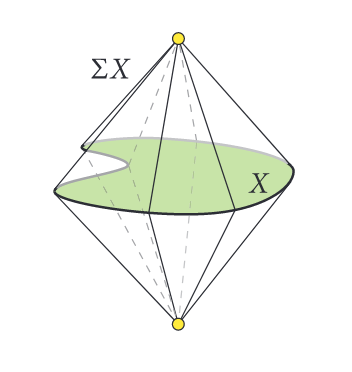
\includegraphics[height=1.5in]{Suspension.png}    
\end{center}



\end{problems}
\end{document}
